\documentclass[12pt,a4paper,titlepage,spanish]{article} 
\usepackage{babel}
\usepackage [T1]{fontenc}
\usepackage [latin1]{inputenc}
\usepackage{graphicx}
\title{Informe Simulaciones TP01 - Prueba del GNA del Lenguaje Java}
\date{14-06-2010}
\author{Vileri�o, Silvio \\6to 1ra \\Turno Noche \\CPU: Intel Core 2 Duo E6600}


\begin{document}
	\maketitle 
	\tableofcontents
	\newpage
	\subsection{Introducci�n}

Esta simulaci�n se desarrolla con el fin de comprobar la calidad del generador de n�meros aleatorios del lenguaje Java, se le realizan varias pruebas, a saber:\\
\begin{itemize}
  \item Se calcula un promedio $ \bar X $ de 1000000 de n�meros generados al azar. El c�lculo es: $$ \bar X= \frac{\displaystyle\sum\limits_{k=1}^{n} {a_k}}{n} ,n = 1000000$$
  \item Se calcula la dispersi�n $ \sigma^2 $ entre cada n�mero generado y el promedio mencionado anteriormente. El c�lculo es: $$ \sigma^2 = \frac{\displaystyle\sum\limits_{i=1}^{n} {(X_i - \bar X)^2}}{n} , n=1000000, \bar X  \longrightarrow \textrm{ promedio} $$ 
  \item Se realiza un histograma en donde se registran la cantidad de n�meros generados entre $ 0.0 $ exclusive y $ 1.0 $ exclusive, en $ 10 $ intervalos de $ 0.1 $
  \item Se calcula $ \bar f = \frac{\displaystyle\sum\limits_{i=1}^{n} {k_i}}{n} , k \longrightarrow \textrm{frecuencia registrada por cada intervalo}, n=10 , \bar f \longrightarrow \textrm{\\frecuencia promedio de los intervalos.}$
	\item Se calcula la dispersi�n $ \sigma^2_{hist} =\frac{\displaystyle{\sum_{i=1}^{n} {(F_i - \bar f)^2}}}{n} , n=100000 $ entre los las frecuencias del histograma y la frecuencia promedio por intervalo.
  \item Se realiza una prueba gr�fica en donde se toman 250000 pares ordenados generados al azar y se dibujan en pantalla en un �rea de $ 500\times 500 $ p�xeles.

\end{itemize}
\newpage	 
\subsection{Resultados}
Luego de realizar las pruebas sobre el cpu mencionado en la primer p�gina, se obtienen los siguientes resultados:\\

\begin{itemize}
	\item Promedio $ \longrightarrow  \bar X = 0.49991325392788877 $ 
 	\item Dispersi�n $ \longrightarrow  \sigma^2 = 0.08347664421385372 $ 
	\item Histograma
		\begin{itemize}
			\item Intervalo $ \left( 0.0 ; 0.1 \right)= 100518 $
			\item Intervalo $ \left[ 0.1 ; 0.2 \right)= 100034 $
			\item Intervalo $ \left[ 0.2 ; 0.3 \right)= 99517 $
			\item Intervalo $ \left[ 0.3 ; 0.4 \right)= 100096 $
			\item Intervalo $ \left[ 0.4 ; 0.5 \right)= 99871 $
			\item Intervalo $ \left[ 0.5 ; 0.6 \right)= 100284 $
			\item Intervalo $ \left[ 0.6 ; 0.7 \right)= 99843 $
			\item Intervalo $ \left[ 0.7 ; 0.8 \right)= 99589 $
			\item Intervalo $ \left[ 0.8 ; 0.9 \right)= 99860 $
			\item Intervalo $ \left[ 0.9 ; 1.0 \right)= 100388 $
			\\
								\begin{center}
									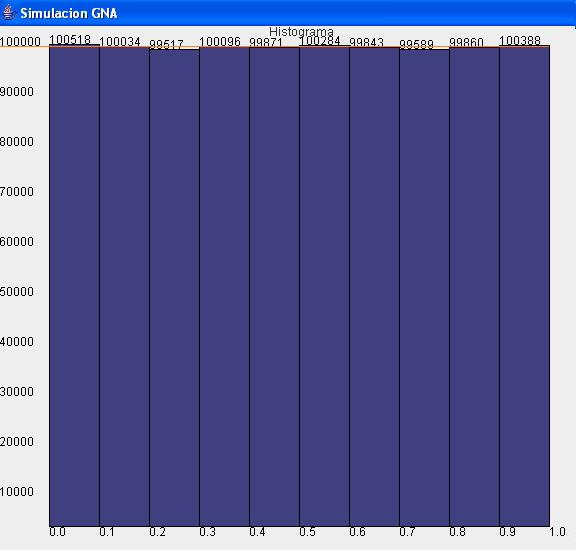
\includegraphics[scale=0.80]{images/histo.JPG}
								\end{center}
				\item Frecuencia Promedio $ \longrightarrow \bar f = 100000 $
				\item Dispersi�n del Histograma $ \longrightarrow \sigma^2_{hist} = 97299.6 $
		\end{itemize}
		\newpage
	\item {Resultado de la prueba gr�fica: \\
	$ 250000 $ puntos al azar en un �rea de $ 500 \times 500 $\\
								\begin{center}
									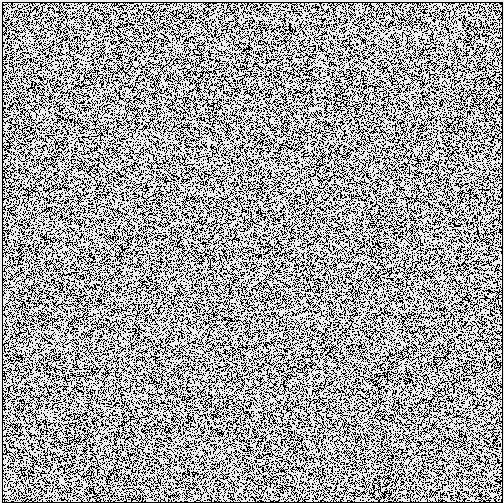
\includegraphics[scale=1.00]{images/testgrafico.JPG}
								\end{center}
								}
\end{itemize}
\newpage
\subsection{Conclusi�n}
Observando los resultados de los an�lisis, se puede concluir que el GNA del lenguaje Java es bueno, dado por las siguientes condiciones cumplidas:
	\begin{itemize}
		\item El promedio $\bar X = 0.49991325392788877 \simeq 0.5 $
		\item La Dispersi�n $ \longrightarrow  \sigma^2 = 0.08347664421385372 $ 
		\item El histograma muestra una planitud en el gr�fico que se traduce en valores $ \simeq $ entre cada intervalo, es decir, valores bien distribuidos entre 0 y 1.
		\item La frecuencia promedio $ \bar f = 100000 $
		\item El test Grafico, que muestra un ruido blanco como una ``lluvia'' de televisi�n, indica que los puntos se han esparcido por todo el �rea de dibujo sin formar figuras ni patrones.
	\end{itemize}

\end{document}
